\documentclass[a4paper,twocolumn]{article}
\usepackage{verbatim}
\usepackage[dvips]{graphicx}
\usepackage{tabularx}

% \newcommand{\intro}[1]{\emph{#1}}


\begin{comment}
\textwidth = 6.5 in
\textheight = 9 in
\oddsidemargin = 0.0 in
\evensidemargin = 0.0 in
\topmargin = 0.0 in
\headheight = 0.0 in
\headsep = 0.0 in
\parskip = 0.2in
\parindent = 0.0in
\end{comment}

\author{Rafael A. Calvo \and Ken Williams}
\title{Automatic Categorization of Announcements on the\\ Australian Stock Exchange}
\begin{document}

\maketitle

\begin{center}
School of Electrical and Information Engineering\\
The University of Sydney\\
Bldg J03, Sydney NSW 2006\\
\{rafa, kenw\}@ee.usyd.edu.au

\end{center}

\section{Abstract}

This paper compares the performance of several machine learning algorithms for the automatic categorization of corporate announcements in the Australian Stock Exchange (ASX) Signal G data stream. The article also describes some of the applications that the categorization of corporate announcements may enable. We have performed tests on two categorization tasks: market sensitivity, which indicates whether an announcement will have an impact on the market, and report type, which classifies each announcement into one of the report categories defined by the ASX. We have tried Neural Networks, a Na\"ive Bayes classifier, and Support Vector Machines and achieved good results.

Section \ref{introduction} of this paper discusses the problem and application domain area, emphasizing the importance of language technologies in the financial information arena. Section \ref{data} describes the Signal G data set.  Section \ref{methods} describes the different machine learning techniques and the categorization framework that we have used to perform these types of categorization tasks. Section \ref{results} describes the quantitative results and section \ref{conclusion} concludes.

\section{Introduction}
\label{introduction}

The Australian Stock Exchange Limited (ASX - http://www.asx.com.au/) operates Australia's primary national stock exchange.  Companies listed on ASX are required under the Listing Rules to make announcements about their activities "in order to ensure a fully informed market is maintained." \cite{asx-reference} In order to guarantee access to this information, stock exchanges such as the ASX publish all recent and historical company announcements.  Thanks to language technologies such as automatic document categorization, these corporate announcements can provide new sources of valuable financial information.

Historically, corporate announcements have provided valuable information to traders and the general public for decades. For this reason these announcements are used by regulators as the main tool to keep the market informed of all important events. The law assumes that these public announcements contain all the information needed by an individual trader to keep a reasonable understanding of what is happening with a particular company. This allows investors to make decisions based on information that is up to date and is equivalent to the information that company insiders might have. There is little doubt about the value of the information contained in these announcements, and there are a number of research groups developing novel applications using this data. These applications include alert systems where brokers receive notification (e.g. over email or SMS) of important announcements, intelligent repositories where the information shown to users is filtered using ``information profiles'' that they can build, and several other applications that require the automatic processing of announcements.  We describe in this article the evaluation of categorization techniques used to build these applications.

The ASX Data Services is a financial information service providing daily market information from the Stock Exchange Automated Trading System (SEATS), ASX futures and the company announcement service.  All daily stock exchange activity is available in different electronic data feeds that the ASX calls ``signals.''  In our work, we have used announcements from the ASX's Signal G, which provides subscribers with company announcements issued by companies or the ASX in accordance with listing rules.

\section{Data Description}
\label{data}

In this paper we assess performance on two tasks: ``report type'' and ``market sensitivity'' categorization. Report type is ``a code to categorize company announcements'' \cite{asx-reference} and may take values like ``annual report'' or ``takeover announcement.'' Market sensitivity is a boolean category indicating whether an announcement contains information that may influence trading in the issuing company. This allows users of this data to select which announcements are critical.

The Signal G documents are created as follows: the ASX's Company Announcement Platform (CAP) receives the announcements produced by organizations (by fax, email or other means), processing and centralizing all the information that is then delivered through the Signal G feed. The processing may include several filtering steps -- for instance, the announcement may be summarized if it is beyond a certain length.  After such processing, each announcement is manually assigned to one of 144 report types, and is classified as either market sensitive or not. From the total 136,630 documents used, 46,530 are marked as sensitive and 90,100 as not sensitive. For this last assignment one or more human classifiers (based on experience) state whether or not the document may have an effect on the value of the share, volume of trading, or other market measurements.  Table \ref{signalg-sensitivity} shows the distribution of documents with respect to the sensitivity category, as well as our split between training and testing documents.

The report type labels are highly skewed across categories.  The most common category, ``XXX,'' contains XXX documents, while the least common category, ``XXX,'' contains only XXX documents.  In order to quantify this skew more precisely, we use a dimensionless statistical measure defined as the standard deviation of a set divided by its mean. For our report type task, the average number of documents per category is XXX and the standard deviation is XXX, giving a skew of XXX.  This quantity allows for comparison with other well-known corpora such as the Reuters-21578 Mod Apt� benchmark corpus, which contains 90 categories, an average of 148.09 documents per category with a standard deviation of 491.84, and thus a skew of 3.32.  A more complete picture of the report type category distribution can be seen in Figure \ref{signalg-reptype}.

Signal G is available to the public, member organizations, and information vendors.  Our data set was supplied by the Capital Markets Collaborative Research Centre.  For future groups who receive permission from the CMCRC to work with this data, we have converted it into an XML format.


\begin{table}
\begin{tabular}{|r|r|r|r|}
\hline
         & Sensitive & Nonsensitive & Total \\
\hline
Training & 32458     & 63067        & 95525 \\
\hline
Test     & 14072     & 27033        & 41405 \\
\hline
Total    & 46530     & 90100        & 136630\\
\hline
\end{tabular}
\caption{Distribution of sensitivity category by number of documents}
\label{signalg-sensitivity}
\end{table}

\begin{figure}
XXX need figure here
\caption{Distribution of report type category by number of documents}
\label{signalg-reptype}
\end{figure}


\section{Methods}
\label{methods}


We have compared three machine learning methods that have provided some of the best performances in other classification tasks \cite{yang:99}: Support Vector Machines (SVM), Na\"ive Bayes (NB), and Neural Networks (NN). It is not possible to describe them thoroughly in this article, so we will only summarize those issues that might be required to reproduce the results.

Our Na\"ive Bayes algorithm is implemented within the AI::Cat\-e\-go\-riz\-er framework, an open source categorization framework written in Perl by Ken Williams.\footnote{Available at \\ http://www.cpan.org/XXX/K/KW/KWILLIAMS/} The framework has been designed to facilitate the construction of new categorization applications following best practices in framework engineering \cite{fayad:99}. Na\"ive Bayes categorizers are one of several well-studied probabilistic categorizers \cite{lewis:98}. Most text categorization research using probabilistic methods uses NB, so a number of authors have described them and shown experimental results on a number of data sets \cite{joachim:98} \cite{yang:99}. 

Support Vector Machines were developed by Vapnik and colleagues during 1995-1996 \cite{cortes:95} \cite{scholkopf:99}. They were first used in document categorization by \cite{joachims:98} \cite{joachims:99} and used by other authors in experimental comparisons with other methods \cite{yang:99}.  Our SVM implementation uses AI::Categorizer for initial text processing, then passes the data through to Weka's SMO (Sequential Minimal Optimization) categorizer for training and testing.

Neural Networks have been widely used and described in the document classification literature. \cite{yang:99} \cite{calvo:00} \cite{calvo:01} The neural network parameters are iteratively adjusted to fit the training data until error stops improving. We have used a backpropagation algorithm that minimizes quadratic error. The input layer has as many units (neurons) as document features retained. The number of hidden units is determined by optimising the performance on a cross-validation set. There is one output unit for each possible category, with activation values between 0 and 1. For each document, the classifier will assign any category whose output unit is greater than 0.5. In our experiment, we used 3-fold cross-validation and averaged the weights of the three resultant neural networks.  Our NN software is the same as in \cite{calvo:00} and \cite{calvo:01}.

Each categorizer was trained on the 95,525 training documents for each task, report type and sensitivity.  For the Neural Network categorizer, XXX training documents were set aside from the training set to function as a validation set when tuning the weights of the network.  The trained categorizers were then evaluated on the 41,405 test documents. Since documents in the test set have not been used to adjust the parameters of the classifier, it is normally assumed that the performance on new data would be similar. 

Table \ref{algos} summarizes the general steps followed in the preparation of the experiments.

\begin{table*}[!b]
\begin{tabularx}{\linewidth}{|r|l|l|X|X|X|}
\hline
& Stopwords & Stemming & Feature Reduction & TF/IDF & Architecture\\
\hline
NN & ??? & Yes & $\chi^2$ & LTC? (Need to find out what this really was) & 1000 features, 50 hidden units \\
\hline
NB & SMART & Yes & DF & TXX & 1000 features \\
\hline
SVM & SMART & Yes & DF & TXX & 1000 features, linear kernel \\
\hline
\end{tabularx}
\caption{Comparative description of algorithms used}
\label{algos}
\end{table*}


\section{Results}
\label{results}


Table \ref{contingency} describes the possible outcomes of a binary classifier.  The ``assigned'' YES/NO results refer to the classifier output and the ``correct'' YES/NO refers to the manual ASX-assigned categories. A perfect classifier would have a value of 0 for $b_j$ and $c_j$.

\begin{table}
\begin{tabular}{|r|r|r|}
\hline
& \multicolumn{2}{|c|}{Correct} \\
\hline
Assigned & YES & NO \\
\hline
YES & $a_j$ & $b_j$ \\
\hline
NO & $c_j$ & $d_j$ \\
\hline
\end{tabular}
\caption{Contingency table for class $j$}
\label{contingency}
\end{table}

Using Table \ref{contingency} we define three performance measures common in the document categorization literature:

\begin{displaymath}
recall = r = \left\{ \begin{array}{ll}
\frac{a}{a+c} & \textrm{if} \, a+c>0 \\
0                  & \textrm{otherwise}
\end{array} \right.
\end{displaymath}

\begin{displaymath}
precision = p = \left\{ \begin{array}{ll}
\frac{a}{a+b} & \textrm{if} \, a+b>0 \\
0                  & \textrm{otherwise}
\end{array} \right.
\end{displaymath}

These two measures contain information about whether classification errors are dominated by false positives or false negatives.  The trade-off between recall and precision can often be controlled by setting a classifier's parameters. Both measures should typically be used to describe the overall performance, as neither is particularly informative by itself. Another common performance measure is the $F_\beta$ measure:

\begin{displaymath}
F_\beta = \frac{(\beta^2 + 1)pr}{\beta^2 p + r}
\end{displaymath}

The most commonly used $F_\beta$ measure in document categorization is $F_1$, which evenly balances precision and recall:

\begin{displaymath}
F_1 = \frac{2pr}{p + r}
\end{displaymath}

When dealing with multiple classes there are two possible ways of averaging these measures, \emph{macro-averaging} and \emph{micro-averaging}. In macro-averaging, one contingency table per class is used, then performance measures are computed on each of them and averaged. In micro-averaging only one contingency table is used; an average of all the classes is computed for each cell and the performance measures are obtained therein. The macro-average weights equally all the classes, regardless of how many documents they contain. The micro-average weights equally all the documents, thus biasing toward the performance on common classes.

Different classifiers will perform differently on common and rare categories. Learning algorithms are trained more often on more populated classes thus risking local overfitting.

\begin{enumerate}

\item Linguistic dimensionality reduction: A list of stopwords \cite{salton:89} was removed from the document collection and the Porter stemming algorithm was applied \cite{manning:99}.
\item Statistical dimensionality reduction: Chi squared, document frequency, and other statistics are often used to reduce the feature vector dimensionality \cite{manning:99} \cite{sebastiani:02}.
\item Vectorization and weighting: The resulting documents were represented as vectors, using TF/IDF weighting \cite{salton:88} \cite{yang:97}. 
\item Architecture: The selected terms were used as input features to the classifier. Some of the algorithms allow several architectures, and the best algorithm was chosen by optimising the results on a cross-validation set. 
\item Training: We generated a cross-validation set randomly. These documents were set aside and the Neural Network was trained on the remaining ones. 

\end{enumerate}

\begin{table}
\begin{tabular}{|c|c|c|c|c|c|c|}
\hline
   & \multicolumn{3}{|c|}{Micro} & \multicolumn{3}{|c|}{Macro} \\
\hline
   & $p$  & $r$  &$F_1$ & $p$  & $r$  & $F_1$ \\
\hline
 NN & 0.89 & 0.89 & 0.89 & 0.88 & 0.88 & 0.88 \\
 NB & 0.83 & 0.84 & 0.83 & 0.90 & 0.90 & 0.90 \\
SVM & 0.82 & 0.82 & 0.82 & 0.80 & 0.79 & 0.80 \\
\hline
\end{tabular}
\caption{Performance for the market sensitivity task}
\label{res:sens}
\end{table}


\begin{table}
\begin{tabular}{|c|c|c|c|c|c|c|}
\hline
   & \multicolumn{3}{|c|}{Micro} & \multicolumn{3}{|c|}{Macro} \\
\hline
   & $p$  & $r$  &$F_1$ & $p$  & $r$  & $F_1$ \\
\hline
NN & 0.87 & 0.71 & 0.78 & 0.45 & 0.34 & 0.37  \\
NB & 0.62 & 0.67 & 0.64 & 0.46 & 0.61 & 0.46  \\
SVM &  &  &  &  &  & \\
\hline
\end{tabular}
\caption{Performance for the report type task}
\label{res:rept}
\end{table}

It is important to note that the performance results are based on comparing the automatic categorization of each document with the tagging of human experts at the ASX. The manual classification is a subjective decision process affected by the ASX�s legal liabilities and the normal human classification disagreements. It has been shown in various studies that there could be considerable variation in the inter-indexer agreement \cite{bruce:98} \cite{brants:00}. For example, in a Reuters news collection correction rates averaged 5.16\% \cite{rose:02} with some editors being corrected up to 77\% of the time. Similar disagreements can be expected in the ASX�s assignments on the Signal G corpus.  In the light of these disagreements we can imagine that there might be a limit to the performance that can be obtained by automatic categorization. 

Figure \ref{histogram} shows a histogram of classes and documents for different performance ranges using the Na\"ive Bayes classifier. It shows how most categories that do well have large number of documents, except for some that have very few documents (fewer than 5). This shows the well-known result that the machine learning algorithms such as Na\"ive Bayes perform better on well-populated categories. Similar results can be obtained for the other classifiers.

\begin{figure}
% 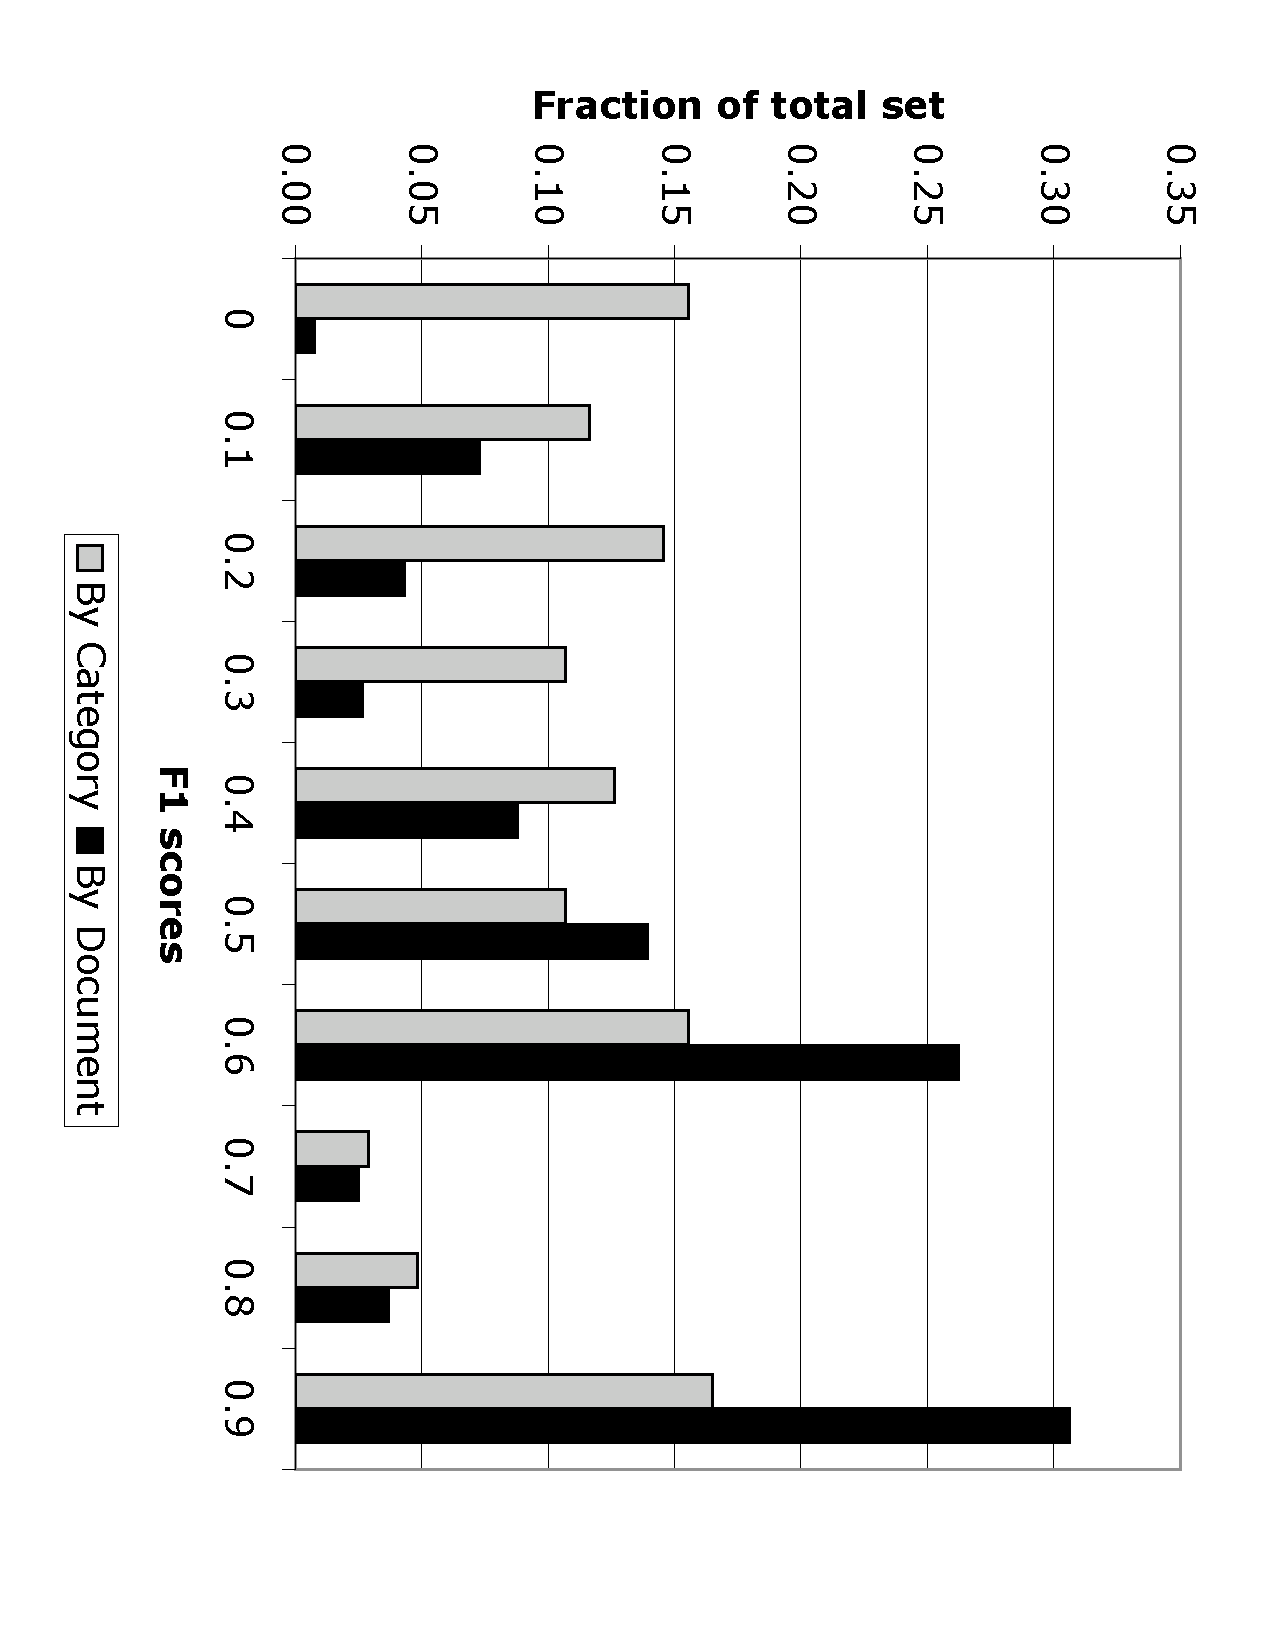
\includegraphics[width=\textwidth]{results.epsf}
\caption{Histogram of report type results for different performance ranges}
\label{histogram}
\end{figure}

\section{Conclusion}
\label{conclusion}


In this paper we have applied several machine learning techniques (Neural Networks, Na\"ive Bayes, and Support Vector Machines) to the categorization of announcements of companies publicly traded by the ASX.  Two tasks were evaluated: the categorization of documents as sensitive or not, and the categorization in one of the 144 report types defined by ASX. The results show that is possible to obtain classifiers with more than 88\% precision and recall on the sensitivity task and 86\% precision, 74\% recall on the report type task.

The results are somewhat better than the ones obtained by several researchers working on the Reuters news cable database \cite{calvo:00} \cite{calvo:01}. This database has fewer categories (90) than the report type task but also fewer documents (10,000). Although it is risky to try to extrapolate the results, we believe that due to the similarity in the documents, other financial databases with documents in English should also have similar performance. Future work includes testing adding statistical feature selection to the classification framework, and improving the efficiency of the algorithms so they can be used for even larger data sets. 

The excellent performance shows the possibility to use these classifiers in commercial applications for both tasks, sensitivity detection and report type categorization.

\section{Acknowledgements}

The authors gratefully acknowledge financial support from the Capital Markets Collaborative Research Centre and the University of Sydney.


\bibliographystyle{plain}
\bibliography{/Users/ken/src/tcframe/ref/TC-references}

\end{document}
